\documentclass{report}
\usepackage{amsmath,amsfonts,amsthm,amssymb}
\usepackage{setspace}
\usepackage{Tabbing}
\usepackage{fancyhdr}
\usepackage{lastpage}
\usepackage{extramarks}
\usepackage{chngpage}
\usepackage{soul,color}
\usepackage{graphicx,float,wrapfig}
\usepackage{tensor}
\usepackage{braket}
\usepackage{lastpage}
\usepackage{subcaption}
\usepackage[procnames]{listings}
\graphicspath{{temika_guide_pics/}}

%Custom coding stuff
\definecolor{keywords}{RGB}{255,0,90}
\definecolor{comments}{RGB}{0,0,113}
\definecolor{red}{RGB}{160,0,0}
\definecolor{green}{RGB}{0,150,0}

\lstset{language=XML,
        basicstyle=\ttfamily\small,
        keywordstyle=\color{keywords},
        commentstyle=\color{comments},
        stringstyle=\color{red},
        showstringspaces=false,
        identifierstyle=\color{green},
        procnamekeys={def,class}}

% In case you need to adjust margins:
\topmargin=-0.45in      %
\evensidemargin=0in     %
\oddsidemargin=0in      %
\textwidth=6.5in        %
\textheight=9.0in       %
\headsep=0.25in         %

\author{by and for the Cicuta Group}
\title{The Temika Guide}
\date{\today}
\begin{document}

\begin{minipage}{\textwidth}
\maketitle
\begin{abstract}
Temika is the home made program that interfaces with the optical tweezers, the Nikon Optical microscopes, and various other equipment of commercial or home-made origin.   Some users purely use the graphical front end, and this contains all the ``physical" buttons on the microscope, plus many settings of the cameras and other equipment.   Importantly, everything in the front end can be coded as a script, for example to automate complex sequences.   It is also possible to implement more complex operations, for example triggered by some event.   Jurij has created this code to capture data and to control a variety of lab equipment; it  has many features and is extremely powerful.    Undoubtedly, it can also be intimidating to use, and it runs in linux which is unfamiliar to some users.\\

This guide focuses on using Temika with the Nikon microscopes, which covers the work of many users.  The first part of this guide will cover how to turn on Temika, see something, record something, and turn the microscope off. The second part will give more detail on the many options, so you can optimize your experiment. The third part will give the rudiments of programming for Temika. The fourth contains descriptions of some commonly done experiments in the group.  \\
\vspace{0.5cm}\\
Special Acknowledgements: Jurij as the author of Temika, Luigi for years of user support, Guil for the first draft of this guide.
\end{abstract}
\end{minipage}

\tableofcontents






\chapter{Temika 101}

\section{Start}

Turn on the microscope connected to your computer.
\\
Once it has booted up, open the terminal, type in \verb|temika|, and press enter.
\\
Temika is now starting up. You may now, if you wish, minimize the terminal window. But do not close it, as this will close Temika. You should now see something like this\\

\begin{figure}[h!]
\centering
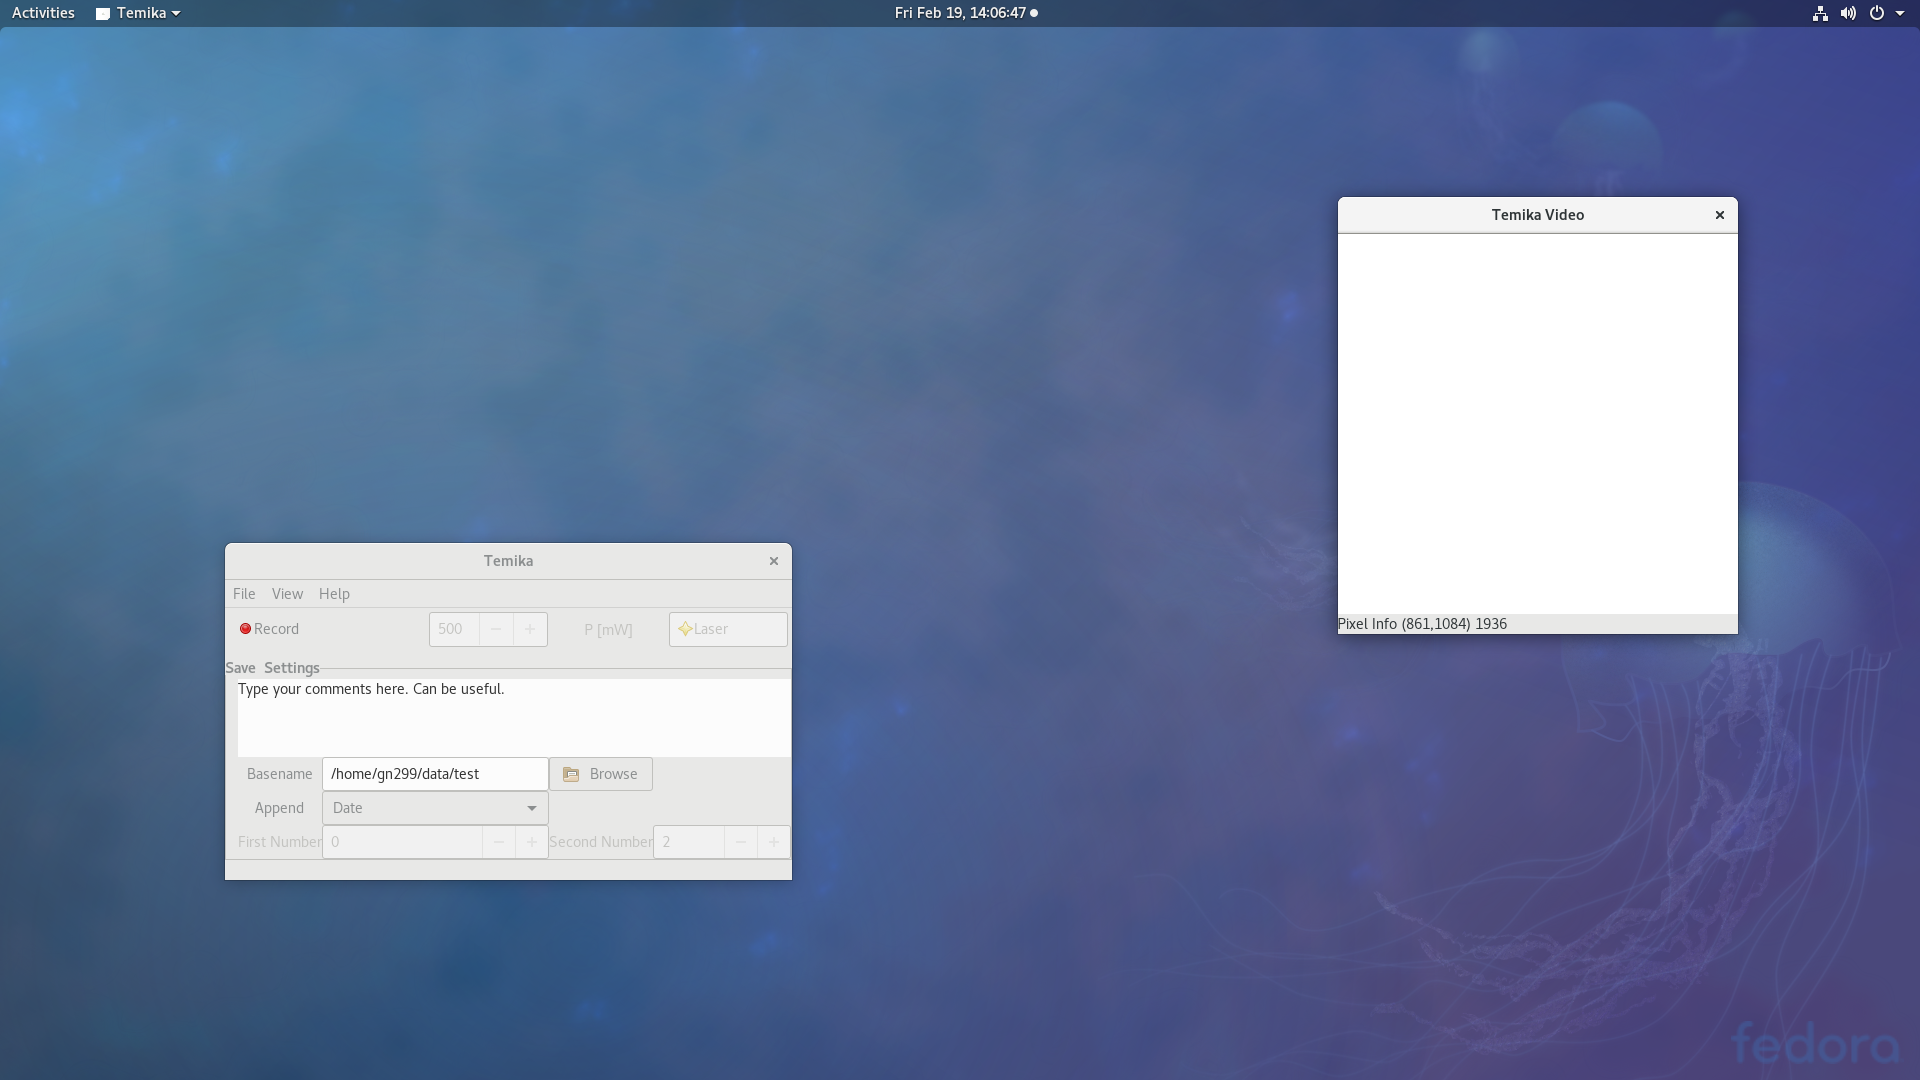
\includegraphics[width=0.75\textwidth]{just_opened}
\end{figure}

This \textbf{Temika} window must also always stay open. Closing it closes the software.\\



\newpage

\section{Display}

The \textbf{Temika Video} window will display the image. At first, it will be all white. To change this, click on \textbf{View} in the \textbf{Temika} window, and select \textbf{Display Settings}.

\begin{figure}[h!]
\centering
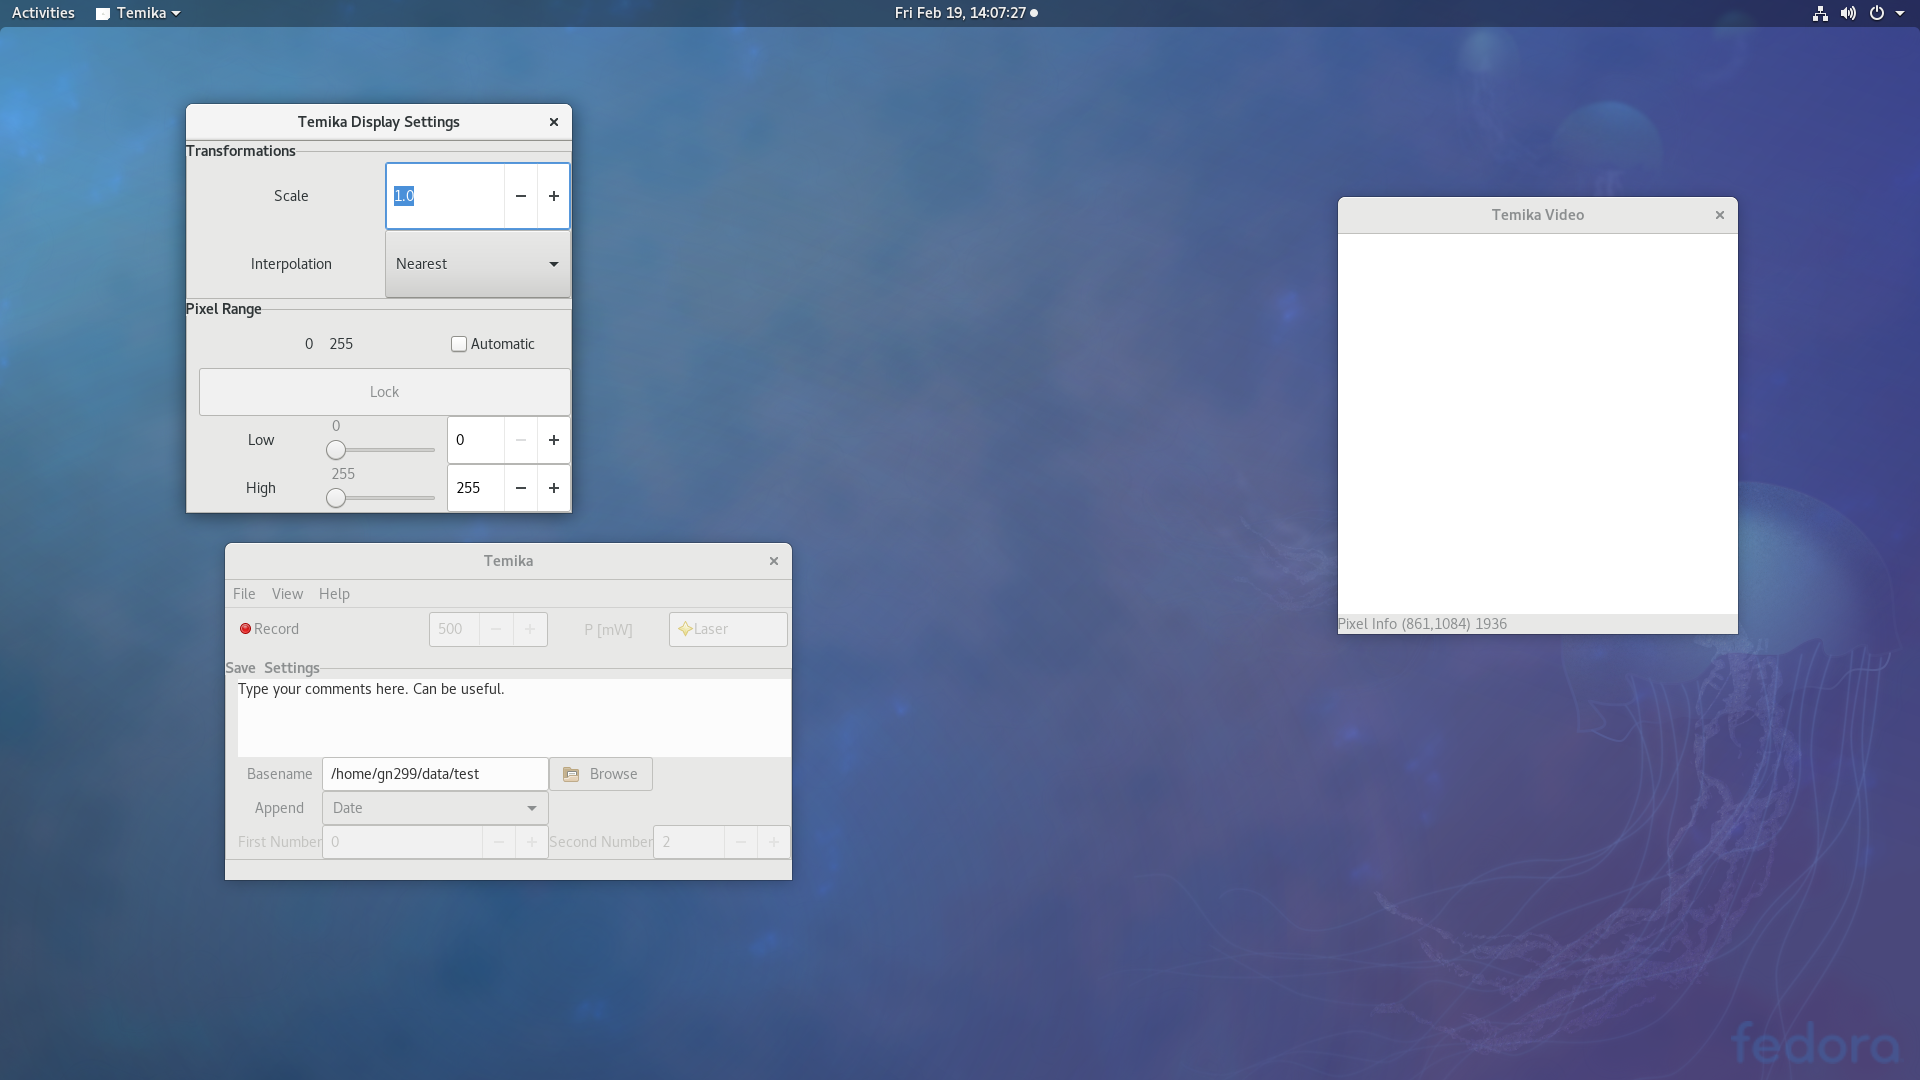
\includegraphics[width=0.75\textwidth]{display}
\end{figure}

Once open, check the \textbf{Automatic} box. The display should now change to display something, most likely static. You may now close the \textbf{Display} window if you wish.





\newpage

\section{Illumination}

Next we will turn on the illumination. Again from the \textbf{View} menu, select \textbf{Illumination}.\\

Temika has two different systems of illumination, depending on which microscope you're using. Look at the pictures below to see which you have:

\begin{figure}[h]
	\begin{subfigure}[b]{0.5\textwidth}
		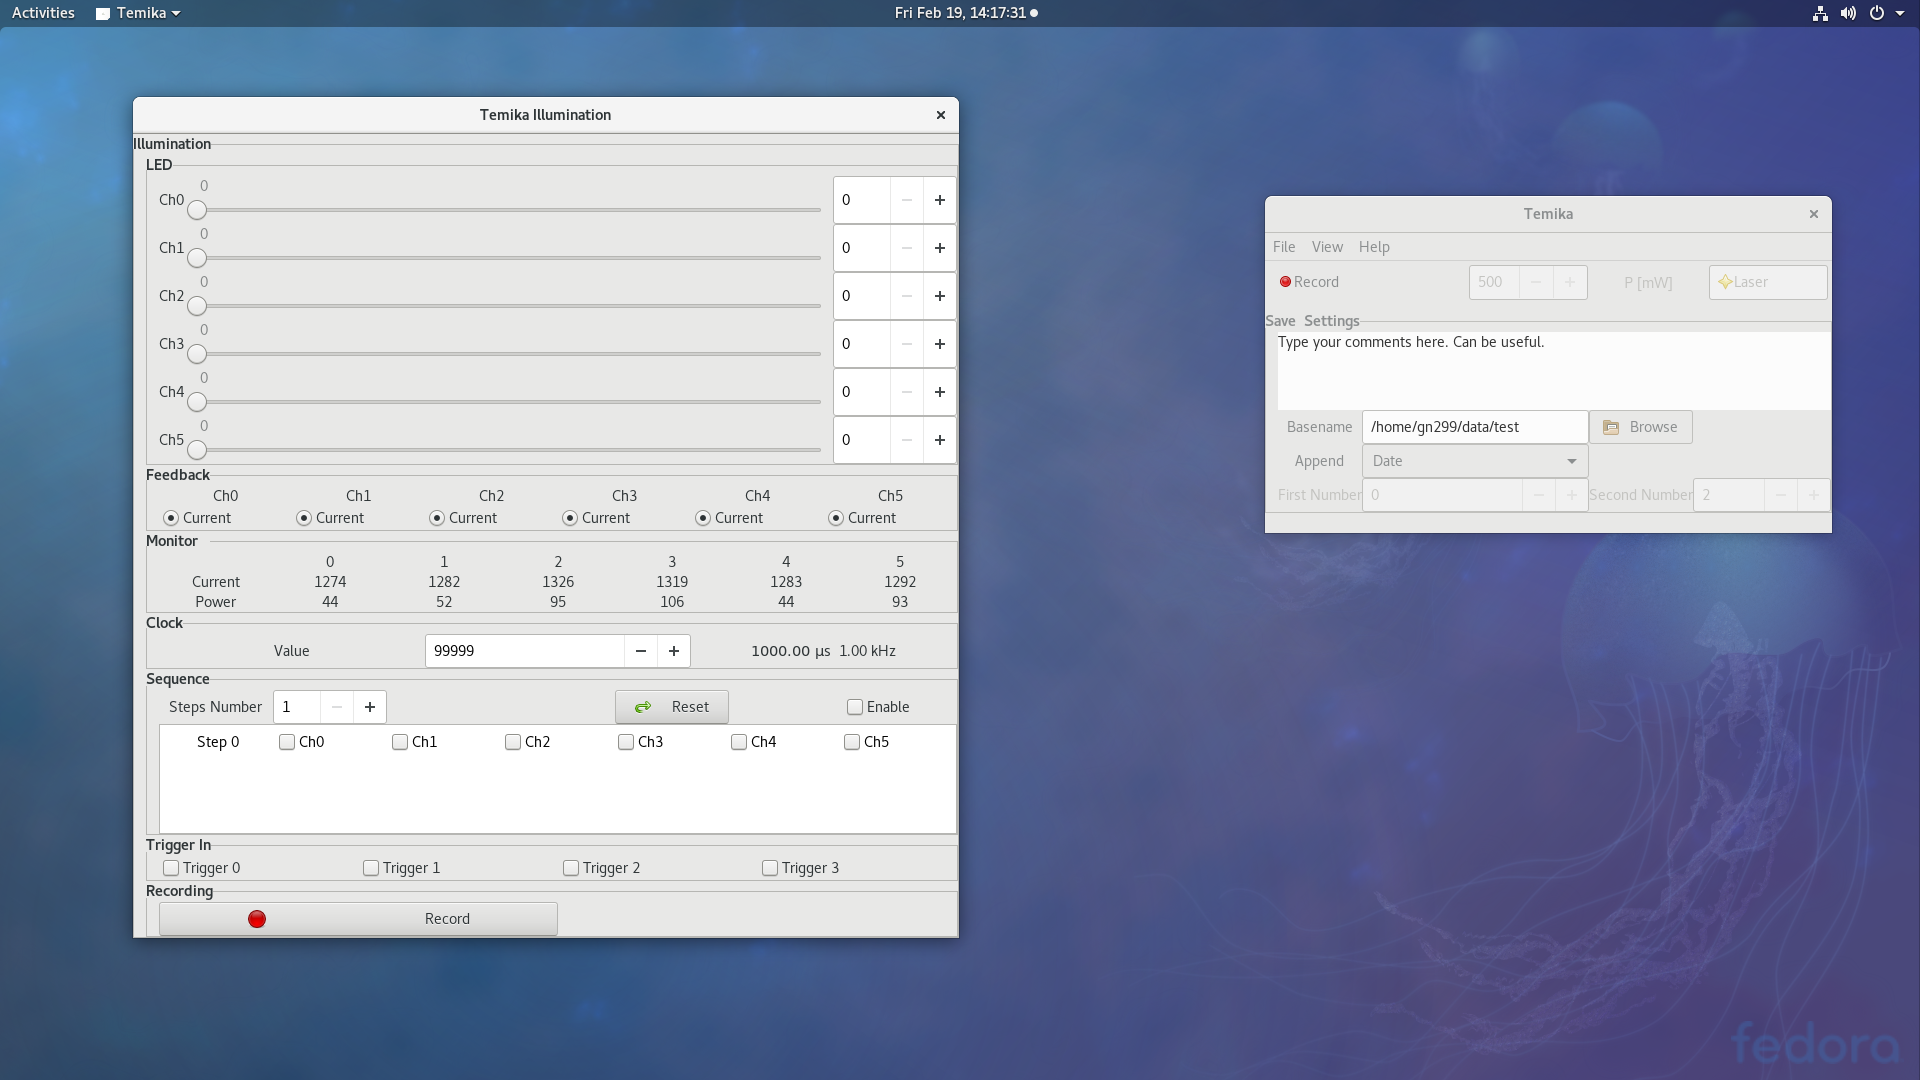
\includegraphics[width=\textwidth]{illumination}
		\caption{6-Channel Illumination}
	\end{subfigure}
	\begin{subfigure}[b]{0.5\textwidth}
		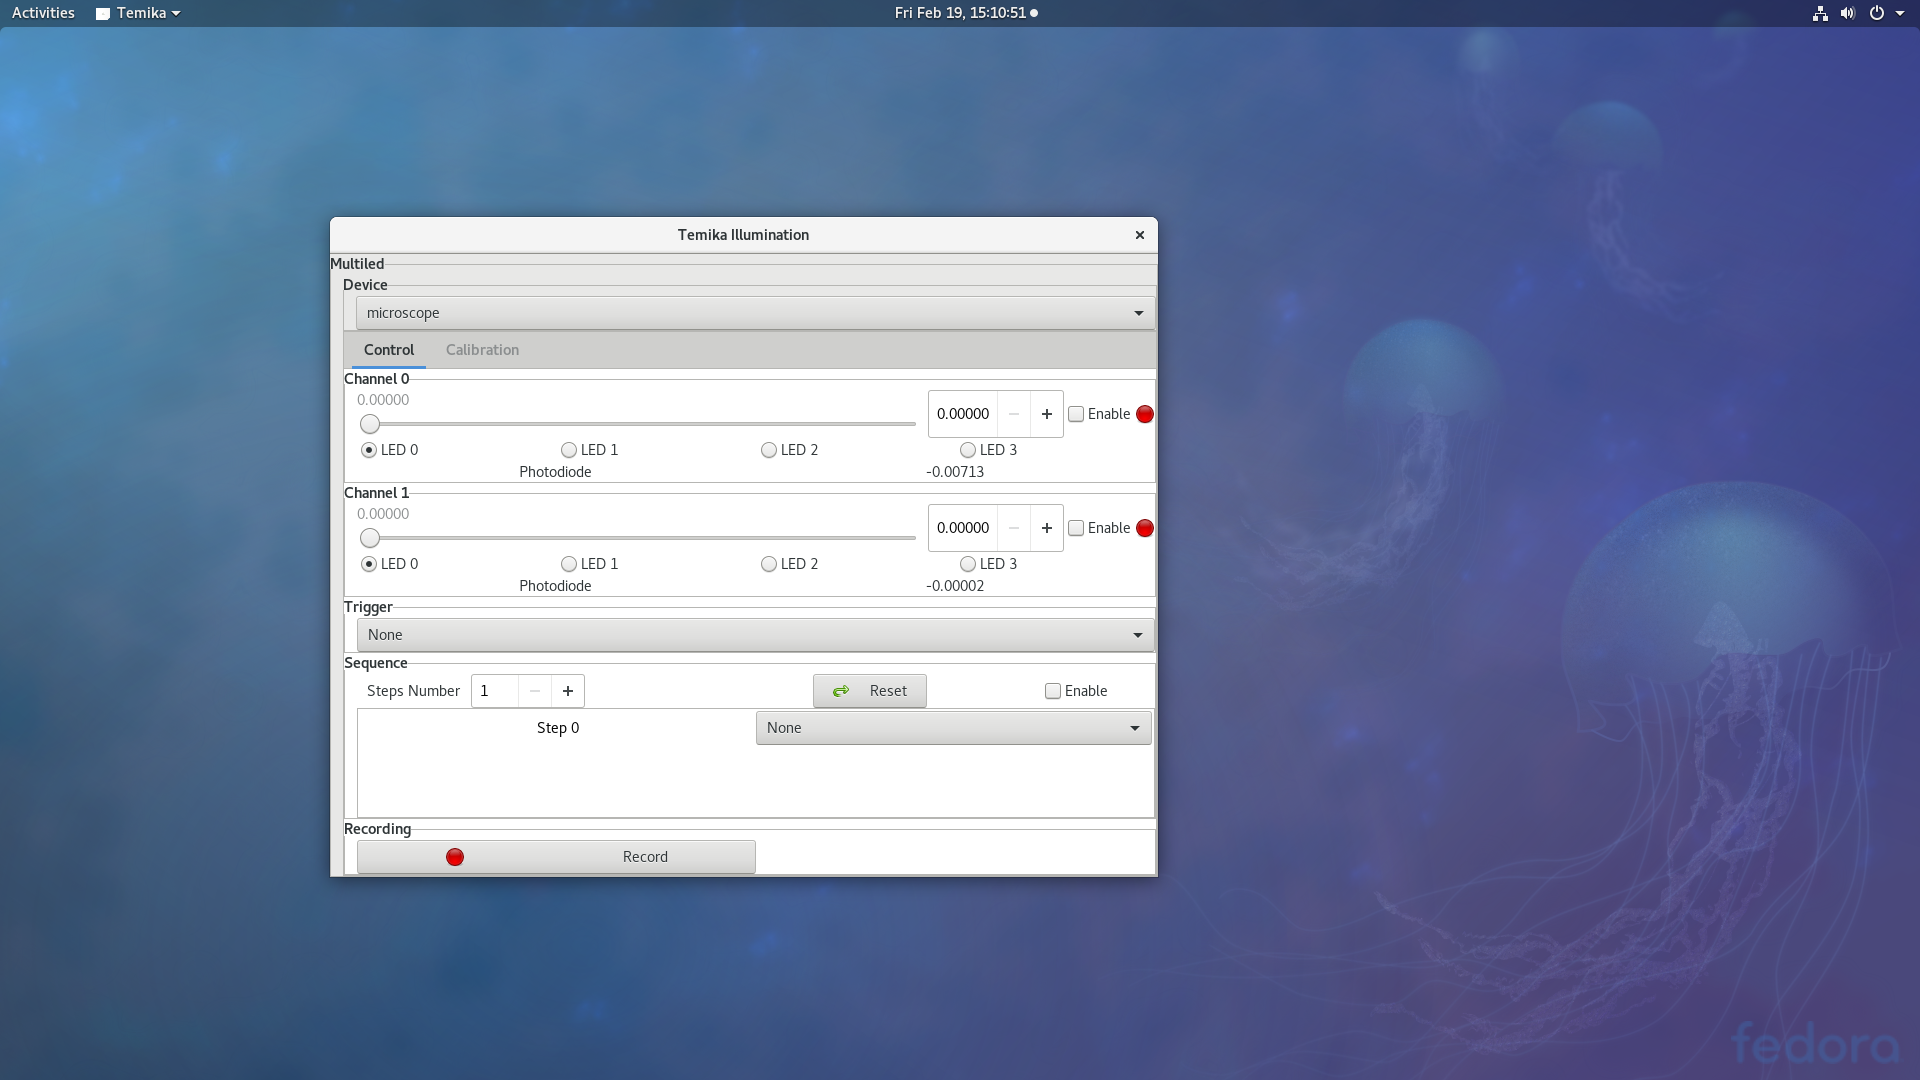
\includegraphics[width=\textwidth]{illumination_led}
		\caption{2-Channel Illumination}
	\end{subfigure}
\end{figure}

Let's see  how to turn on a single channel (i.e. color) at a time.


\subsection{6-Channel Illumination}

You have six channels available to you. These will correspond to different wavelengths of light, and may illuminate the sample from above or below. You will have to either know what each channel corresponds to, or you will have to try them and see.\\

Under the \textbf{LED} panel, pick your channel of choice and slide the intensity dial to the right some amount. You can adjust this later. Nothing should happen yet.\\

Under the \textbf{Sequence} panel, click \textbf{Enable}. Then, below, check the box corresponding to your channel of choice.\\

Finally, under the \textbf{Trigger In} panel, you will have to select the correct trigger\footnote{See appendix Illumination Trigger for more information}. This will depend on the camera you are using, and how it is connected. It is almost always Trigger 0 or Trigger 1. Once you have selected the correct one, you should see the illumination.\\

Common reasons why you aren't seeing anything include:
\begin{itemize}
	\item The channel you picked is not visible (UV or IR).
	\item The light is very dim.
	\item The channel you picked is for fluorescence and needs the right filter cube, or the aperture is shut.
	\item You have not clicked \textbf{Enable}.
	\item You have picked the wrong trigger. Try all four to be sure.
\end{itemize}

%\newpage

\subsection{2-Channel Illumination}

You have two channels available to you, each of which has four different LEDs. These will correspond to different wavelengths of light, and may illuminate the sample from above or below. You will have to either know what each channel corresponds to, or you will have to try them and see.\\

Under either the \textbf{Channel 0} or \textbf{Channel 1} panels, slide the intensity dial to the right some amount, and click the LED of choice. You can adjust this later. Nothing should happen yet.\\

Under the \textbf{Trigger} panel, you will have to select the correct trigger \footnotemark[\value{footnote}]. This will depend on the camera you are using, and how it is connected. It is almost always External 0 or External 1.\\

Under the \textbf{Sequence} panel, click \textbf{Enable}. Then, below, from the dropdown menu, select the option corresponding to your channel and LED of choice. You should see the illumination.\\

Common reasons why you aren't seeing anything include:
\begin{itemize}
	\item The channel you picked is not visible (UV or IR).
	\item The light is very dim.
	\item The channel you picked is for fluorescence and needs the right filter cube, or the aperture is shut.
	\item You have not clicked \textbf{Enable}.
	\item You have picked the wrong trigger. Try all three to be sure.
\end{itemize}

\newpage


\section{Camera}

Next we will adjust the camera. From the \textbf{View} menu, select \textbf{Camera Control}.\\

You should now see the camera settings. However, what you see now will depend on what cameras are installed. Most likely, you will see a window like this:

\begin{figure}[h!]
\centering
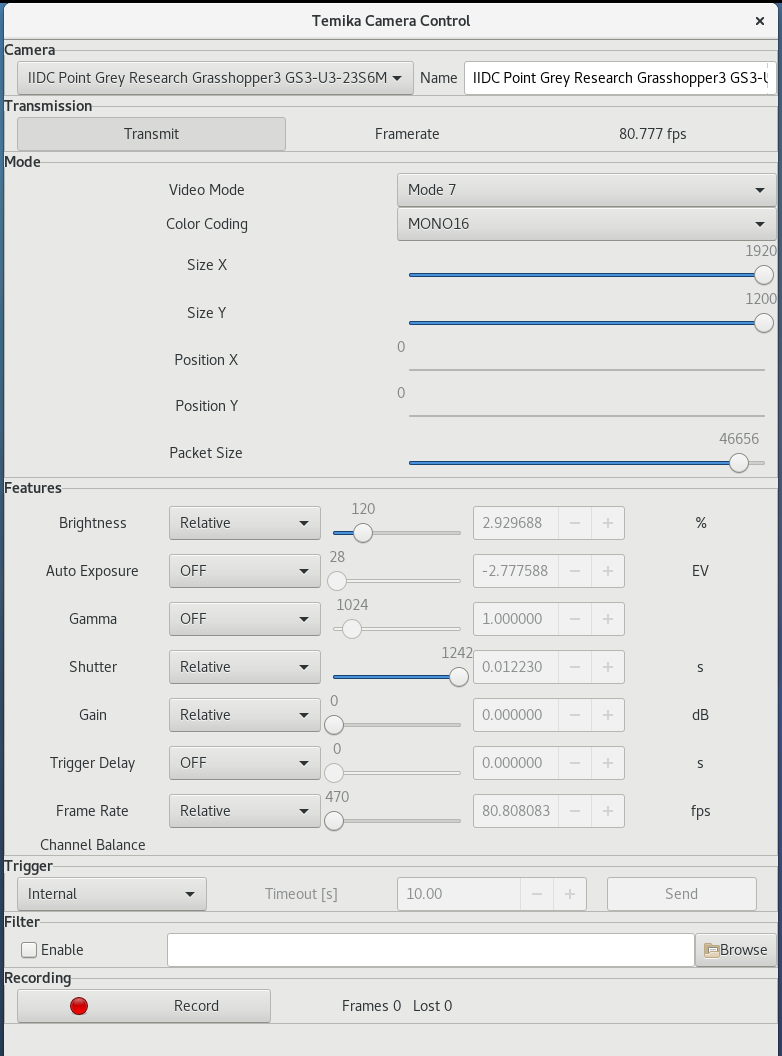
\includegraphics[width=0.75\textwidth]{grasshopper}
\end{figure}

This is the \textbf{Temika Camera Control} for the IIDC Point Grey Research Grasshopper3. This camera suffices for most uses---Imaging live cells, most fluorescent signals---though it may struggle with very weak signals, where someting like the Andor iXon3 will perform better.\\

The Grasshopper has many settings. We will only roughly explain how to set these. For more details, consult the Advanced Topics section~\ref{Grasshopper Features}.\\

First, make sure \textbf{Video Mode} is set to \textbf{Mode 7}, and \textbf{Color Coding} to \textbf{MONO16}, to give the best color depth.\\

Also make sure that, in the \textbf{Trigger} panel, \textbf{Internal} is selected.\\

At this point, you will want to adjust three properties, depending on your sample:
\begin{enumerate}
	\item The framerate, which is displayed on the top-right corner
	\item The exposure time, which is set and displayed under \textbf{Shutter time}
	\item The image quality
\end{enumerate}

While in practice it is not difficult to tune all of these, it takes just a few moments of playing around. To do so, adjust the following---and \emph{only} the following---options:
\begin{enumerate}
	\item \textbf{Size X} and \textbf{Size Y}: This will decrease the image area, increasing the frame rate. If you need very high framerates, decreasing X and Y is a great idea.
	\item \textbf{Gain}: Increase this if you still cannot see your signal clearly (note, there will be more camera noise).
	\item \textbf{Shutter}: Increasing the exposure time will make the image brighter, but the trade off is blurring from dynamics. Iin some cases (e.g. flickering) you want small exposure times.
	\item \textbf{Framerate}: This will ---surprise!--- change the framerate.
\end{enumerate}

All of this is complicated by \textbf{Packet Size}, a mysterious and powerful parameter\footnote{``But what is Packet Size?'' Jurij is the only one who knows.}. If you find that you cannot get the framerate you want, change the packet size. This will change the ranges of available framerates and exposure times.





\newpage

\section{Microscope}

Next we will adjust the microscope settings. From the \textbf{View} menu, select \textbf{Microscope}.\\

\begin{figure}[h!]
\centering
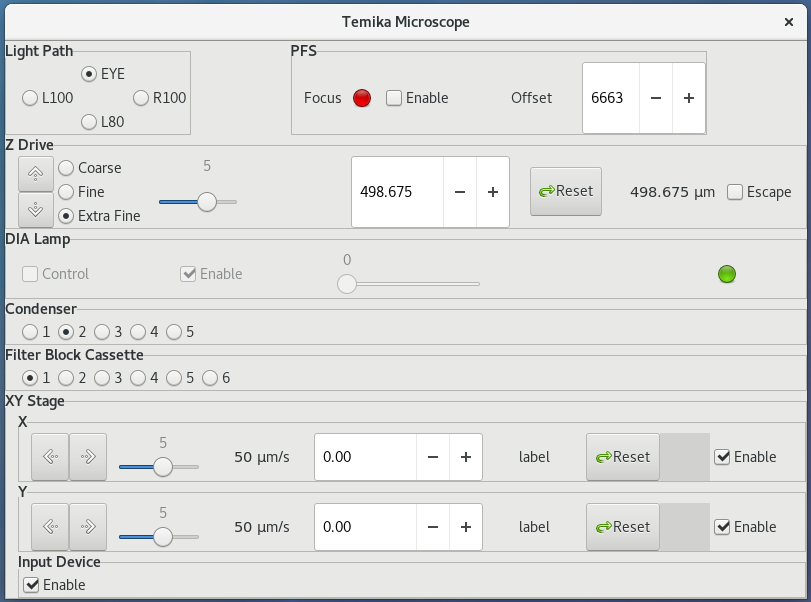
\includegraphics[width=0.75\textwidth]{microscope}
\end{figure}

Under \textbf{Light Path}, make sure that the correct port is selected for your camera. If at this point you see nothing on your camera, this is likely the issue!\\

Once you have focused on your sample using the microscope's knobs, you can turn on the Perfect Focus System, which will keep your sample in focus. To do this, check \textbf{Enable} under \textbf{PFS}. You will then be able to control the focus using the attached PFS focus dial.\\

It is possible that PFS does not work, in which case it will not enable. There are many possible reasons. The two most common are that: the coverslip is of the wrong thickness or has something obstructing it, like a plastic film; or  the objective you are using is not the correct one for the turret. If trouble persists, seek Jurij.\\

You will also be able to change the microscope's filter block and condenser. Make sure these are set correctly for what you need.\\



\newpage

\section{Recording}

Now, assuming you have done everything correctly and you have also loaded and adjusted the microscope correctly, you are ready to record. First, feel free to type a comment in the comment box, and to change the basename of the file (the default is ``test'', and you will kick yourself later for not changing this to something more specific!).\\

To record, press the \textbf{Record} button in the \textbf{Temika} window. Press it again to stop recording. The videos should be saved in the directory next to \textbf{Basename}.



\newpage

\section{Quitting}

Once you are done, turn off the illumination


\section{Saving out of the lab}
Deprecated - you attach an external drive. This is fast, but drives get lost or corrupted fairly easily.\\

Preferred - type \verb|cifs| in a  terminal,  you can then access BSS common folders such as \textbf{space} or \textbf{cicutagroup} from the computer \textbf{sf3}, then insert your BSS password. Moving files in this way takes longer but gets your files to a disk array that is almost failsafe, and can be accessed from anywhere on the internet.\\

Whichever way you have moved the data out of the lab, once you know it is safely saved elsewhere, delete the copy saved on the lab computer.   You will otherwise put other people's experiment (or your own future experiment) at risk of not having space to save.    Data is precious - keep it in two places, for example your own desktop and one of the NAS spaces \textbf{space} or \textbf{cicutagroup}.


\section{How to use .movie files?}
Temika saves files in a raw format called the ``movie''.   This is a very flexible format, with useful metadata for example on timing and frame sizes.   You can do things like change the frame size during your recording (although this would make conversions more complicated later!).


On the linux computers in the labs there are two commands to export the videos into uncompressed tiff images: movie2tiff and movie2tiff\verb|_|color.

There are also  Luigi’s files for doing manipulations of .movie into other formats (mp4, load into MATLAB or ImajeJ/Fiji, but they do not work with colour formats): http://people.bss.phy.cam.ac.uk/~lf352/      If your data analysis is going to be in Matlab, you can load the .movie directly there without other conversions. Code to do that in C++ also exists (Jurij, and Part III project of George Haskell 2021) and the same could be done in Python.\\

Note 1 - it is a good idea to keep one copy of the original .movie data.   You can compress it into zip or tar at no loss.

Note 2 -  many of the conversions from .movie will lose data quality (compression, or depth of bits) and many will lose important info like the timestamp (framerate) - so convert only if necessary.      It is obviously a good idea to have small, compressed, exports of the parts of movies that you want to show in presentations.







\newpage

\chapter{Temika and the connected hardware}

Now that you know how to do very basic things with Temika, here we will go into more detail into the many options Temika offers.

%\newpage

\section{Triggers}

Triggers can seem a bit confusing. Essentially, the two process of turning on the illumination and recording a frame on the camera have to be precisely synchronized, and triggers do that.     Both the camera and the illumination need to be triggered, which is why both have trigger options.\\

\subsection{Camera triggers}

The camera trigger determines when a frame is taken. Of course, each camera is different, but they will likely have an \textbf{Internal} option. This means that the camera will be ``triggered'' by its own, internal clock. Therefore, at fixed intervals, the camera's clock will send a trigger to the camera (i.e. itself) that says, ``Take a frame!'' When you're recording or watching a video, this is the setting you'll want to use.\\

There will also be a \textbf{Software} option. This means that the trigger will come from Temika. If you switch to this option, the video should immediately stop, since the internal clock is no longer triggering the camera. You'll also notice the \textbf{Send} button, on the same row as the trigger options, will no longer be greyed out. Press this button to send a trigger to the camera. The camera image should quickly update. The use of the \textbf{Software} is that it allows you to take snapshots at discrete and user-defined times. It is particularly useful when scripting. The \textbf{Timeout} options determines how long the program will wait for the camera to return back a frame, before it gives up and counts the frame as lost. There is almost never a reason to change this.\\

To clear a common point of confusion, if you press \textbf{Record} while the trigger is in \textbf{Software} mode, you will see the recording time ticking down, while the image stays still. Is the computer recording a bunch of the same frames? No, which you can easily verify by looking at the number of frames at the very bottom of the camera window. Only when you hit send, will a frame actually be recorded to the \verb|.movie| file.

In addition to these, there can  be other ``external'' triggers, and these will differ from camera to camera. Cameras are able to be triggered by other devices, by sending some kind of signal to the camera. Since we never use ``external'' triggers, I can't say anything about these. Unless you have a very good reason, it's best to avoid these ``external'' triggers.\\

\subsection{Illumination triggers}

The illumination trigger determines when the light source is on. The light source must be triggered for it to work. Each illumination source has multiple ports. Some of these are connected to the cameras being used. Thus, when a camera is triggered---by its own internal clock, for example, or the software---the camera sends its own signal to the illumination source, triggering it. In that way, the illumination can be ON only when the camera is acquiring a frame. You work out which camera is connected to which trigger  by trial-and-error, or looking at the physical connections, or asking Jurij. \\

The 6-Channel light source has four triggers: \textbf{Trigger 0}, \textbf{Trigger 1}, \textbf{Trigger 2}, and \textbf{Trigger 3}. You need to know which trigger corresponds to which camera. With the 6-Channel light source, you can also choose multiple triggers, which will trigger the light if any of the selected triggers go off. Additionally, there is \textbf{None}, so that the light source stays OFF.\\

The 2-Channel light source has three triggers: \textbf{External 0}, \textbf{External 1}, and \textbf{External 2}, as well as \textbf{None}, and works very similarly. Unlike the 6-Channel case, only one trigger can be selected at a time.




\newpage

\section{Illumination sequences}

Illumination sequences are a way to have multiple illumination sources come ON  in a predictable way. As example, this allows you to record alternating frames with fluorescence and brightfield, or cycle through different fluorescent channels.\\

In fact, you are always using an illumination sequence, though it might be a sequence with only one step. Just as easily, you can add more steps. For either the 6-Channel or the 2-Channel illumination, increase or decrease the number of steps under \textbf{Sequence}. For each step, select the channel(s) that you would like to have active at that moment. Lastly, the \textbf{Reset} button return the sequence to the beginning.\\


\section{Recording the illumination state}



Unfortunately, the saved \verb|.movie| file does not keep track of where we are in the sequence, so there is  no absolute way to extract this information from the \verb|.movie| file. In practice, you might  design things so that this is obvious from the image.\\

You can however record the illumination state as well in its own file by hitting \textbf{Record} in the illumination window. This saves a time series of the current\footnote{Jurij - check this is correct?} through each channel of the illumination source. The resulting file can be rather large, and matching  it to the \verb|.movie| file can be a bit of a pain, but if knowing exactly what the illumination source was doing and when is important, this can be invaluable.




\newpage

\section{Temperature}


todo




\newpage

\section{Grasshopper Features}\label{Grasshopper Features}

The Grasshopper Camera, also know as the IIDC Point Grey Research Grasshopper3, is one of our more common cameras and has many features.


Crucial to what is going to be possble are two things: (1) the physical properties of the camera sensor, which will have some level of noise (i.e. sensitivity), readout time, number and size of pixels;   (2) the transfer of information from camera to computer.   There is very little that you can do on (1), except study what cameras we have, and which ones are worth trying. There are also new cameras coming to market all the time, and everyone should keep their eyes open!.   (2) also depends on hardware components, but is something on whcih you have a lot more control.   The key concept is the bandwidth.  Taking from \footnote{https://www.flir.co.uk/support-center/iis/machine-vision/application-note/usb-3.1-multiple-camera-setup/}: To calculate your bandwidth requirements, use your required resolution, frame rate, and pixel format (bytes per pixel) in the following equation:\\
Height x Width x Frame Rate x Bytes per Pixel = Bandwidth in MB\\

For example:\\
Camera model: FL3-U3-13S2M-CS\\
Resolution: 1328 x 1048\\
Frame rate: 60 FPS\\
Pixel format: Mono16\\
Bandwidth = 1328 x 1048 x 60 x 2 = 167 MB/s\\

You can also turn this equation around to work out a framerate, based on a bandwidth.

The  bandwidth of  USB 3.1  is approximately 450 MB/s, but peak performance can vary.   Knowing how much data you are importing can also be important in terms of bandwidth saving to hard drive, and having enough space on the drives. A typical 7200 RPM HDD will deliver a read/write speed of 80-160MB/s. A typical SSD will deliver read/write speed of between 200 MB/s to 550 MB/s.

\begin{figure}[h!]
\centering
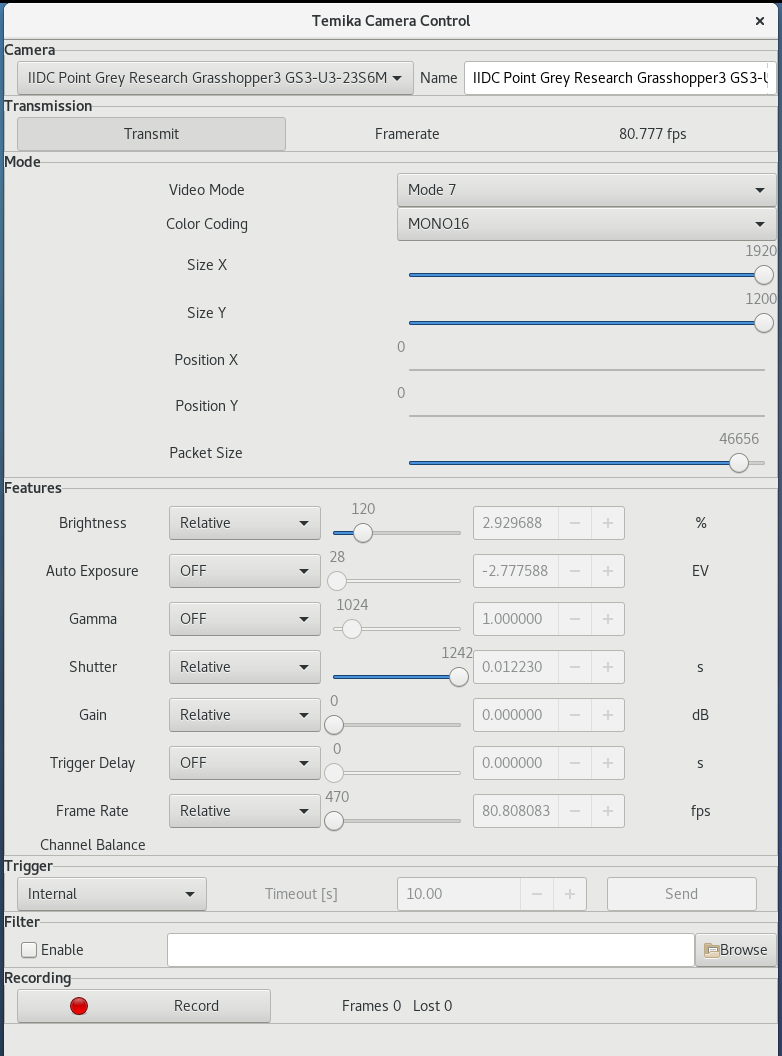
\includegraphics[width=0.60\textwidth]{grasshopper}
\end{figure}

\textbf{Video Mode} sets the camera's mode of operation. \textbf{Mode 7} is for low noise and is generally recommended. If you have trouble achieving a high enough framerate with \textbf{Mode 7}, try switching to \textbf{Mode 0}. This will give a higher frame rate, though at a slightly lower signal-to-noise ratio. There is also \textbf{Mode 1}. This bins 2x2 groups of pixels. \textbf{Mode 1} is not recommended!\\

\textbf{Color Coding} determines the color depth of the image. The image is digitized by a 12-bit analog-to-digital converter. Therefore, the full depth of color is given by \textbf{MONO12}. However, 12-bit encoding is rather unusual compared to 8-bit and 16-bit, which is why \textbf{MONO16} exists and is recommended: It is the same information as \textbf{MONO12}, with an extra four $0$'s in the least-significant parts of the number. Transmitting these four ``redundant'' bits makes the transfer just a tad slower, but it does make your images easier to open. \textbf{MONO8} is certainly faster than both previous options, but it does come with a decrease in depth. I am a bit unclear at what \textbf{RAW8} does, since the raw image should be 12-bits.\\

\textbf{Size X and Size Y} are self-explanatory. The use of decreasing the image size is always that the framerate is greatly increased.\\

\textbf{Position X and Position Y}, too, are self-explanatory. If you have a dirty sensor or unever illumination, it makes sense to use it.\\

\textbf{Packet Size} This is a number, in bytes, that is the amount of information the camera sends to the CPU as a packet. If it's too high, can result in dropped frames and other problems.   Decreasing this is one way to decrease framerate.\\

\textbf{Brightness} scales the values of the pixels. It really should never be played with.\\

\textbf{Auto Exposure} should be left off, unless you have a very good reason! It changes the camera exposure based on how much light it is receiving. This would naturally be a bad idea for most experiments.\\

\textbf{Gamma} is gamma correction. Essentially, it takes each pixels intensity values and raises it to the power of gamma. This is great for photography, not great for experiments. Also should be left off. \\

\textbf{Shutter} changes the time the camera exposes for. Feel free to dial this up if you have a relatively static image, but if you have something that has a lot of dynamic information, such a flickering membrane, you'll want to keep this low.\\

\textbf{Gain} increases the gain in the image. This is the electronic amplification in the camera.  This makes each pixel more sensitive to light, which increases the signal but also the noise. Feel free to turn this up.\\

\textbf{Trigger Delay}  Not clear what this does or when it might be useful, and should be left off.\\

\textbf{Frame Rate} changes the frame rate, within the constraints given by the other settings.\\







\newpage

\chapter{Temika working for You: Scripts, Feedback, and Filter programming}

Temika becomes an incredibly powerful tool once you learn to program for it. There many  ways to program for Temika: An xml-based scripting language for automating simple, non-interative tasks; a much more powerful C-based feedback system that can react to the image on the camera; and a filter system that can modified the displayed frame. We will describe each of these.

\section{XML-scripting}

The XML script is perfect for simple tasks that need to be repeated the same a large number of times.  You can use your own favourite code (Matlab, Python, whatever) to actually write out the potentially quite long XML script.    The  main limitations of this approach are that it cannot react to any inputs, and that it lacks any of the basic functionalities of a language: There are no control sequences and no declaration of variables.\\

Attached to this script is an xml file called \verb|script_language.xml|. This is the Rosetta Stone of the Temika xml script, handed down to use from Jurij. Consult it if you have any doubts.\\

Every XML script has the following format:

\lstinputlisting{xml_scripts/script_skeleton.xml}

Inside the \verb|<temika>| bracket we put all of our commands. With one exception, everything is done sequentially. I will now go over basic commands.\\

todo - very useful!!!





\newpage

\subsection{example: 6-Channel Illumination}

\lstinputlisting{xml_scripts/6_channel_illumination_language.xml}

Selecting channels can be a bit tricky. You must convert the channels to a hexadecimal number. So, all six channels off is equal to $000000 = 0x00$. Turning on channels $0$, $1$, and $5$ is equal to $100011 = 2^0 + 2^1 + 2^5 = 1 + 2 + 32 = 35 = 0x23$. If this is too complicated, and you only want to use a single channel at a time, refer to this list:

Channels:\\
All off = 0x00\\
0 on = 0x01\\
1 on = 0x02\\
2 on = 0x04\\
3 on = 0x08\\
4 on = 0x10\\
5 on = 0x20\\

Likewise, for the triggers:\\
All off = 0x0\\
0 on = 0x1\\
1 on = 0x2\\
2 on = 0x4\\
3 on = 0x8\\

\newpage

\subsection{example:  2-Channel Illumination}

\lstinputlisting{xml_scripts/2_channel_illumination_language.xml}

\section{Feedback programs}

todo



\section{Filters}

todo





\newpage


\chapter{Applications/Protocols}

\section{Flickering - Guil}
 todo

\section{Malaria tweezing - Emma Jones}

Optical tweezers set up for malaria sample
Emma: Sample - Mix purified Shizonts with 0.05\% HCT fresh blood in complete media, 200$\mu$l. Use a SecureSeal hybridization chamber (SecureSeal; Grace Bio-Labs, Bend). Coat the cover slip with 5ul of poly(l-lysine)-graft-poly(ethylene glycol) (PLL-g-PEG) (SuSoS AG, Dubendorf, Switzerland) at 0.5 mg/mL concentration.

 Lens  60x water objective (Plan Apo VC 60x 1.20 NA water objective, Nikon).
    Frame rate: 20 frames/sec
    Pixel size:  0.0973$\mu$m


\begin{figure}[h]
		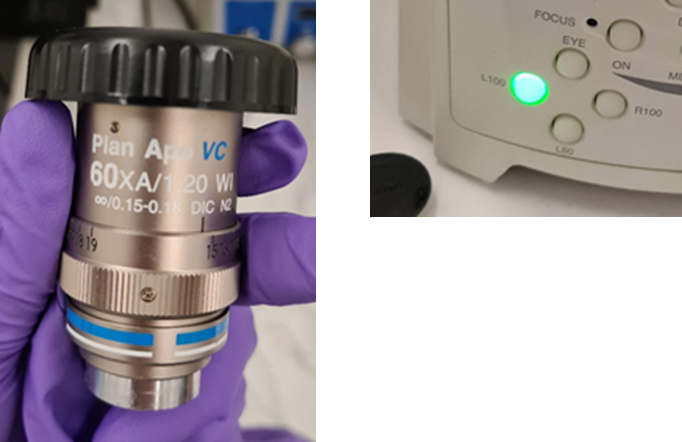
\includegraphics[width=6cm]{fig1}
		\caption{Microscope - Emma settings}
\end{figure}

\begin{figure}[h]
		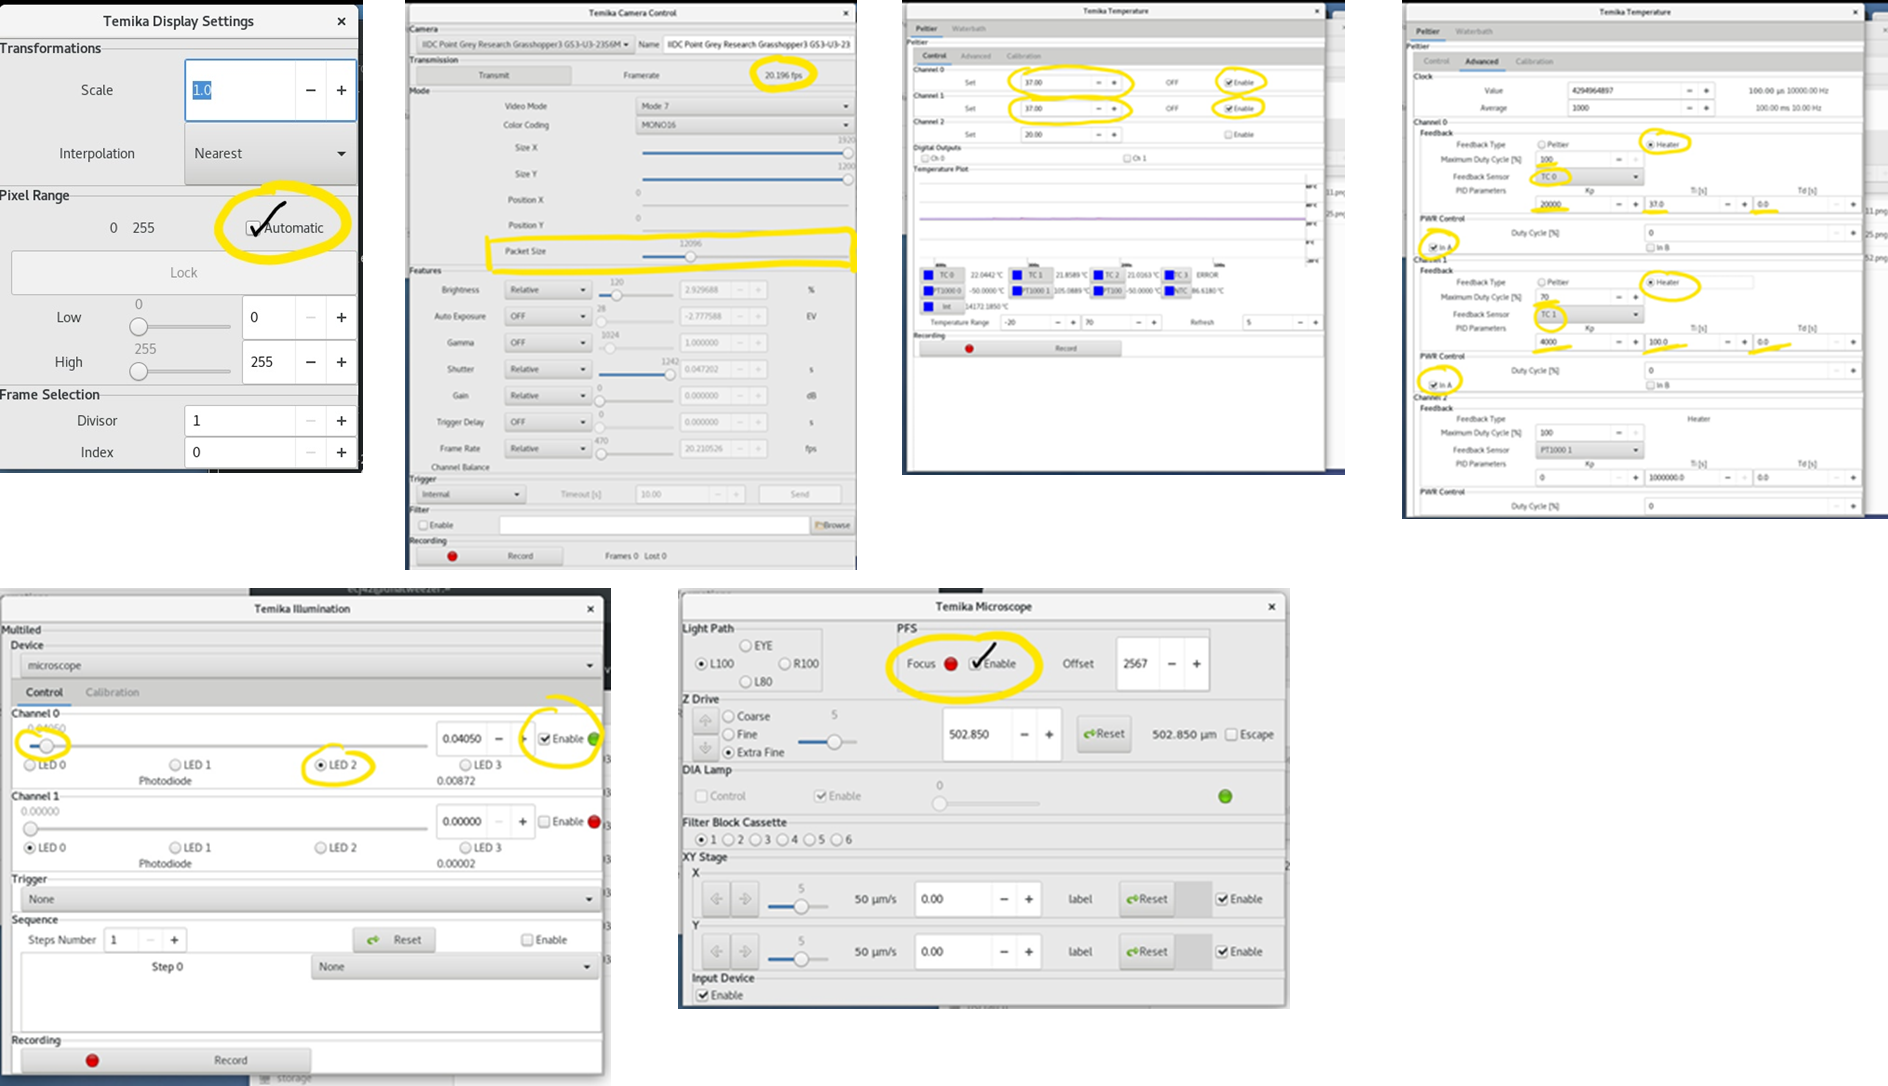
\includegraphics[width=\textwidth]{fig2}
		\caption{Temika - Emma settings}
\end{figure}


1.    Set the room alarm if using malaria sample ;    Turn on Microscope, laser and heater at wall;    Login to computer and open temika.

2.    Microscope - Adjust the lens position to P APO VC 60X/1,20, using the buttons on the left of the microscope. Attach the Plan Apo Vc 60xA/1.20 WI .   Set path to L-100.

3.    Microscope/Temperature - Attach the heat collar to the lens, connected to `output 1' and attach the temperature probe wire to the side of the lens with aluminium tape.


4.    Microscope/Temperature - Tape the sample onto the heated holder (Glass over slip side down), tape temperature `probe 0' to the same side. Connect the holder to `socket 0'.


5.    Microscope/Sample - Put a drop of water on the lens and then place sample on.



6.    Temika terminal –     display settings: set to automatic;    Camera Controller: adjust the frame rate to 20 fps;     Temperature: adjust the settings so that temperature set to 3$^o$C;
Illumination;

7.    Microscope – focus on the RBC

8.    Temika terminal and  Microscope: turn on the perfect focus

9.    Temika terminal – Traps – right click on image and create traps, then scroll when clicked on them to turn up strength.


\section{Bacteria microcolonies and/or microfluidics  - Leonardo}
Bacteria imaging in 3rd microscope todo

\section{Algae imaging in alga microscope  - who?}
todo

\section{Cilia transwells  - Ricardo}
todo





\chapter{Other}

\section{When to call Jurij}
Jurij will have helped you startup, and is generally more than happy to know how you proceed with your Temika/imaging adventures.   If you have advanced requests, desires to go beyond what you are currently getting,  talk to Jurij and/or Pietro.   \\

On a day-to-day basis, get hold of Jurij for the following:
\begin{itemize}
  \item Things that look like faults or bugs
  \item Booting/rebooting the linux computers in case of freezes or shutdown  (you might succeed yourself, but he needs to know when things crash in order to troubleshoot for the future)
  \item  Creating user accounts
  \item   Misalignment of tweezers
  \item  Changes in the illumination modules and filtersets (unless you have been shown)
\end{itemize}










\end{document}
